\chapter{Neural Networks}
\label{chap-neural_networks}
You've probably been
hearing a lot about ``neural networks.''   Now that we have several
useful machine-learning concepts (hypothesis classes, classification,
regression,  gradient descent, regularization, etc.) we are
well equipped to understand neural networks in detail.

This is, in some sense, the ``third wave'' of neural nets.  The basic
idea is founded on the 1943 model of neurons of McCulloch and Pitts
and the learning ideas of Hebb.  There was a great deal of excitement, but
not a lot of practical success:  there were good training methods
(e.g., perceptron) for linear functions, and interesting examples of
non-linear functions, but no good way to train non-linear functions
from data.   Interest died out for a while,  but was re-kindled in the
1980s when several people \note{As with many good ideas in science,
  the basic idea for how to train non-linear neural networks with
  gradient descent was independently developed by more than one
  researcher.} came up with a way to train neural networks with
``back-propagation,'' which is a particular style of implementing
gradient descent, that we will study here.  By the mid-90s, the
enthusiasm waned again, because although we could train non-linear
networks, the training tended to be slow and was plagued by a problem
of getting stuck in local optima.   Support vector machines ({\sc svm}s)
that use regularization of high-dimensional hypotheses by seeking to maximize
the margin, and kernel methods that are an efficient and beautiful way of
using feature transformations to non-linearly transform data into a
higher-dimensional space, provided reliable learning methods with
guaranteed convergence and no local optima.

However, during the {\sc svm} enthusiasm, several groups kept working
on neural networks, and their work, in combination with an increase in
available data and computation, has made them rise again.  They have
become much more reliable and capable, and are now the method of
choice in many applications.   There are many, many \note{The number
  increases daily, as may be seen on {\tt arxiv.org}.} variations of
neural networks, which we can't even begin to survey.  We will study
the core ``feed-forward'' networks with ``back-propagation''
training, and then, in later chapters, address some of the major
advances beyond this core.

We can view neural networks from several different perspectives:
\begin{description}
  \item{\bf View 1}: An application of stochastic gradient descent for
        classification and regression with a potentially very rich
        hypothesis class.
  \item{\bf View 2}: A brain-inspired network of neuron-like computing
        elements that learn distributed representations.
  \item{\bf View 3}: A method for building applications that make
        predictions based on huge amounts of data in very complex domains.
\end{description}

We will mostly take view 1, with the understanding that the techniques
we develop will enable the applications in view 3.  View 2 was a major
motivation for the early development of neural networks, but the
techniques we will study do not \note{Some prominent
  researchers are, in fact, working hard to find analogues of these methods in
  the brain.} seem to actually account for the biological learning
processes in brains.

\section{Basic element}
The basic element of a neural network is a ``neuron,'' pictured
schematically below.  We will also sometimes refer to a
neuron as a ``unit'' or ``node.'' \index{neuron}
\begin{center}
  \begin{tikzpicture}[main node/.style={thick,circle,font=\Large}]
    \node[main node,draw](sum) at (0,0) {$\sum$};
    \node[main node](x1) at (-2,1) {$x_1$};
    \node[main node](dots) at (-2,0) {$\vdots$};
    \node[main node](xm) at (-2,-1) {$x_m$};
    \coordinate (w0) at (0,-1.5);
    \node[main node, draw] (f) at (2,0) {$f(\cdot)$};
    \node[main node] (y) at (4,0) {$a$};

    \draw[->, above right] (x1) -- node {$w_1$} (sum);
    \draw (dots) -- node {} (sum);
    \draw[->, below right] (xm) -- node {$w_m$} (sum);
    \draw[above right] (w0) node {$w_0$} --  (sum) ;
    \draw[->, above] (sum) -- node (z) {$z$} (f);
    \draw[->, above] (f) -- (y);

    \node[black!70] (inp) at ($(xm) + (0,-1.5)$) {input};
    \node[black!70] (pre) at ($(z) + (0,1)$) {pre-activation};
    \node[black!70] (out) at ($(y) + (0,1)$) {output};
    \node[black!70] (act) at ($(f) - (0,1.5)$) {activation function};

    \draw[->,black!70] (inp) -- (xm);
    \draw[->,black!70] (pre) -- (z);
    \draw[->,black!70] (out) -- (y);
    \draw[->,black!70] (act) -- (f);
  \end{tikzpicture}
\end{center}

It is a non-linear function of an input vector  $x \in \R^m$ \note{Sorry
  for changing our notation here.  We were using $d$ as the dimension
  of the input, but we are trying to be consistent here with many
  other accounts of neural  networks.  It is impossible to be
  consistent with all of them though---there are many different ways
  of telling this story.} to a single output value $a \in \R$.  It is
parameterized by a vector of {\em weights} $(w_1, \ldots, w_m) \in
  \R^m$ and an {\em offset} \note{This

  should remind you of our $\theta$ and $\theta_0$ for linear models.} or {\em threshold} $w_0 \in \R$. In order for the neuron to be non-linear, we also specify an {\em
    activation function} $f : \R \rightarrow \R$, which can be the
identity ($f(x) = x$, in that case the neuron is a linear function of $x$), but can also be any other function, though we
will only be able to work with it if it is differentiable.

The function represented by the neuron is expressed as:
\[a = f(z) = f\left(\left(\sum_{j=1}^m x_jw_j\right) + w_0\right) = f(w^Tx + w_0)\;\;.\]

Before thinking about a whole network, we can consider how to train a
single unit. Given a loss function $\mathcal{L}(\text{guess}, \text{actual})$
and a dataset $\{(\ex{x}{1}, \ex{y}{1}), \ldots,
  (\ex{x}{n},\ex{y}{n})\}$, we can
do (stochastic) gradient descent, adjusting the weights
$w, w_0$ to minimize
\[J(w, w_0) = \sum_{i} \mathcal{L}\left(\text{NN}(\ex{x}{i}; w, w_0), \ex{y}{i}\right)\;,\]
where $\text{NN}$ is the output of our single-unit neural net for a given input.

We have already studied two special cases of the neuron:
linear logistic classifiers (LLCs) with NLL loss and regressors with
quadratic loss! The activation function for the LLC is $f(x) =
  \sigma(x)$ and for linear regression it is simply $f(x) = x$.
\question{
  Just for a single neuron, imagine for some reason, that we decide to
  use activation function $f(z) = e^z$ and loss function $\mathcal{L}(\text{guess}, \text{actual}) = (\text{guess} - \text{actual})^2$.  Derive a gradient descent update for $w$ and $w_0$.
}
\section{Networks}
Now, we'll put multiple neurons together into a {\em network}.  A
neural network \index{neural network}in general takes in an input $x \in \R^m$ and generates
an output $a \in \R^n$.  It is constructed out of multiple neurons;
the inputs of each neuron might be elements of $x$ and/or outputs of
other neurons.   The outputs are generated by $n$ {\em output units}.  \index{neural network!output units}

In this chapter, we will only consider {\it feed-forward} networks\index{neural network!feed-forward network}.  In
a feed-forward network, you can think of the network as defining a
function-call graph that is {\em acyclic}:  that is, the input to a
neuron can never depend on that neuron's output.  Data flows one way,
from the inputs to the outputs, and the function computed by the
network is just a composition of the functions computed by the
individual neurons.

Although the graph structure of a feed-forward neural network can really be
anything (as long as it satisfies the feed-forward constraint), for
simplicity in software and analysis, we usually organize them into
  {\em layers}\index{neural network!layers}.   A layer is a group of neurons that are essentially
``in parallel'':  their inputs are outputs of neurons in the previous
layer, and their outputs are the input to the neurons in the next
layer.   We'll start by describing a single layer, and then go on to
the case of multiple layers.

\subsection{Single layer}
A {\em layer} is a set of units that, as we have just described, are
not connected to each other. The layer is called
  {\em fully connected}\index{neural network!fully connected} if, as in the diagram below, 
  all of the inputs
% the inputs to each unit in the layer are the same 
(i.e., $x_1, x_2, \ldots x_m$ in this
case) are connected to every unit in the layer.  A layer has input $x \in \R^m$ and output (also known as
  {\em activation}) $a \in \R^n$.

\begin{center}
  \begin{tikzpicture}[main node/.style={circle}]
    \coordinate (soff) at (0,1.4);
    \node[main node,draw](s1) at ($2*(soff)$) {$\sum$};
    \node[main node,draw](s2) at (soff) {$\sum$};
    \node[main node,draw](s3) at (0,0) {$\sum$};
    \node[main node](sdots) at ($(0,0)-(soff)$) {$\vdots$};
    \node[main node,draw](sn) at ($(0,0)-2*(soff)$) {$\sum$};

    % inputs
    \coordinate (x) at (-2,0);
    \coordinate (xoff) at (0,1);
    \node[main node](x1) at ($(x) + 1.5*(xoff)$) {$x_1$};
    \node[main node](x2) at ($(x) + .5*(xoff)$) {$x_2$};
    \node[main node](xdots) at ($(x) - .5*(xoff)$) {$\vdots$};
    \node[main node](xm) at ($(x) - 1.5*(xoff)$) {$x_m$};

    % activations
    \coordinate (foff) at (1.5,0);
    \node[main node, draw](f1) at ($(s1) + (foff)$) {$f$};
    \node[main node, draw](f2) at ($(s2) + (foff)$) {$f$};
    \node[main node, draw](f3) at ($(s3) + (foff)$) {$f$};
    \node[main node] at ($(sdots) + (foff)$) {$\vdots$};
    \node[main node, draw](fn) at ($(sn) + (foff)$) {$f$};

    % outputs
    \node[main node](y1) at ($(s1) + 2*(foff)$) {$a_1$};
    \node[main node](y2) at ($(s2) + 2*(foff)$) {$a_2$};
    \node[main node](y3) at ($(s3) + 2*(foff)$) {$a_3$};
    \node[main node] at ($(sdots) + 2*(foff)$) {$\vdots$};
    \node[main node](yn) at ($(sn) + 2*(foff)$) {$a_n$};

    % arrows
    \foreach \b in {(s1), (s2), (s3), (sn)}
    \foreach \a in {(x1), (x2), (xm)}
    \draw[->] \a -- \b;
    \foreach \x/\y/\z in {(s1)/(f1)/(y1), (s2)/(f2)/(y2),
        (s3)/(f3)/(y3), (sn)/(fn)/(yn)}{
        \draw[->] \x -- \y;
        \draw[->] \y -- \z;
      }
    %\foreach \x in {(s1), (s2), (s3), (sn)}
    %  \draw \x -- +(0,-.65);
    \node[main node, ,below left] (weights) at ($(xm)!0.5!(sn)$)
    {$W,W_0$};
  \end{tikzpicture}
\end{center}
Since each unit has a vector of weights and a single offset, we can
think of the weights of the whole layer as a matrix, $W$, and the
collection of  all the offsets as a vector $W_0$.
If we have $m$ inputs, $n$ units, and $n$ outputs, then
\begin{itemize}
  \item $W$ is an $m\times n$ matrix,
  \item $W_0$ is an $n \times 1$ column vector,
  \item $X$, the input, is an $m \times 1$ column vector,
  \item $Z = W^T X + W_0$, the {\em pre-activation}, is an $n \times
          1$ column vector,
  \item $A$, the {\em activation}, is an $n \times 1$ column vector,
\end{itemize}
and the output vector is
\[A = f(Z) = f(W^TX + W_0)\;\;.\]
The activation function $f$ is applied element-wise to the
pre-activation values $Z$.

% What can we do with a single layer?  We have already seen single-layer
% networks, in the form of linear separators and linear regressors.  All
% we can do with a single layer is make a linear hypothesis.~\note{We
%   have used a step or sigmoid function to transform the linear output
%   value for classification, but it's important to be clear that the
%   resulting {\em separator} is still linear.} The whole reason for
% moving to neural networks is to move in the direction of {\em
%     non-linear} hypotheses.  To do this, we will have to consider
% multiple layers, where we can view the last layer as still being a
% linear classifier or regressor, but where we interpret the previous
% layers as learning a non-linear feature transformation $\phi(x)$,
% rather than having us hand-specify it.

\subsection{Many layers}
A single neural network generally combines multiple layers, most
typically by feeding the outputs of one layer into the inputs of
another layer.

We have to start by establishing some nomenclature.  We will use $l$
to name a layer, and let $m^l$ be the number of inputs to the layer
and $n^l$ be the number of outputs from the layer.  Then, $W^l$ and
$W^l_0$ are of shape $m^l \times n^l$ and $n^l \times 1$,
respectively. Note that the input to layer $l$ is the output from
layer $l-1$, so we have $m^l= n^{l-1}$, and as a result $A^{l-1}$ is
of shape $m^l \times 1$, or equivalently $n^{l-1} \times 1$. Let $f^l$
be the activation function\index{activation function} of layer
$l$. \note{It is technically possible to have different activation
  functions within the same layer, but, again, for convenience in
  specification and implementation, we generally have the same
  activation function within a layer.}Then, the pre-activation outputs
are the $n^l \times 1$ vector
\[Z^l = {W^l}^TA^{l-1} + W^l_0\]
and the activation outputs are simply the $n^l \times 1$ vector
\[A^l = f^l(Z^l)\;\;.\]

Here's a diagram of a many-layered network, with two blocks
for each layer, one representing the linear part of the operation and
one representing the non-linear activation function.  We will use this
structural decomposition to organize our algorithmic thinking and
implementation.

\begin{center}
  \begin{tikzpicture}
    \coordinate (x) at (0,0);
    \node[inner sep=0em] (w1) at (1.7,0)
    {\begin{tabular}{c} $W^1$ \\ $W^1_0$\end{tabular}};
    \node[inner sep=1em] (f1) at ($2*(w1)$) {$f^1$};
    \node[inner sep=0em] (w2) at ($3*(w1)$)
    {\begin{tabular}{c} $W^2$ \\ $W^2_0$\end{tabular}};
    \node[inner sep=1em] (f2) at ($4*(w1)$) {$f^2$};
    \node (dots) at ($5*(w1)$) {$\cdots$};
    \node[inner sep=0em] (wL) at ($6*(w1)$)
    {\begin{tabular}{c} $W^L$ \\ $W^L_0$\end{tabular}};
    \node[inner sep=1em] (fL) at ($7*(w1)$) {$f^L$};
    \coordinate (y) at ($8*(w1) - (.3,0)$);

    \draw[->] (x) -- node[above] {$X = A^0$} (w1);
    \draw[->] (w1) -- node[above] {$Z^1$} (f1);
    \draw[->] (f1) -- node[above] {$A^1$} (w2);
    \draw[->] (w2) -- node[above] {$Z^2$} (f2);
    \draw[->] (f2) -- node[above] {$A^2$} (dots);
    \draw[->] (dots) -- node[above] {$A^{L-1}$} (wL);
    \draw[->] (wL) -- node[above] {$Z^L$} (fL);
    \draw[->] (fL) -- node[above] {$A^L$} (y);

    \draw [decorate,decoration={brace,mirror,amplitude=10pt}]
    ($(w1) + (-.4, -.7)$) -- node[yshift=-1.8em] {layer 1}
    ($(f1) + (.4,-.7)$);
    \draw [decorate,decoration={brace,mirror,amplitude=10pt}]
    ($(w2) + (-.4, -.7)$) -- node[yshift=-1.8em] {layer 2}
    ($(f2) + (.4,-.7)$);
    \draw [decorate,decoration={brace,mirror,amplitude=10pt}]
    ($(wL) + (-.4, -.7)$) -- node[yshift=-1.8em] {layer $L$}
    ($(fL) + (.4,-.7)$);


    \foreach \point in {w1, f1, w2, f2, wL, fL}{
        \draw ($(\point) + (-.3,-.5)$) rectangle ($(\point) + (.3,.5)$);
      }
  \end{tikzpicture}
\end{center}

\section{Choices of activation function}

There are many possible choices for the activation function.  We will
start by thinking about whether it's really necessary to have an $f$
at all.

What happens if we let $f$ be the identity?  Then, in a network with
$L$ layers (we'll leave out $W_0$ for simplicity, but keeping it
wouldn't change the form of this argument),
\[A^L = {W^L}^T A^{L-1} =
    {W^L}^T {W^{L-1}}^T \cdots {W^1}^T X\;\;.\]
So, multiplying out the weight matrices, we find that
\[A^L = W^\text{total}X\;\;,\]
which is a {\em linear} function of $X$!
Having all those layers did not change the representational
capacity of the network: the non-linearity of the activation function
is crucial.
\question{Convince yourself that any function representable by any
  number of linear layers (where $f$ is the identity function) can be
  represented by a single layer.}

Now that we are convinced we need a non-linear activation, let's
examine a few common choices.
These are shown mathematically below, followed by plots of these functions.
\begin{description}
  \item{\bf Step function:} \index{activation function!step function}
        $$\text{step}(z) =
          \begin{cases}
            0 & \text{if $z<0$}  \\
            1 & \text{otherwise}
          \end{cases}$$
  \item{\bf Rectified linear unit (ReLU):} \index{activation function!ReLU}
        $$\text{ReLU}(z) =
          \begin{cases}
            0 & \text{if $z<0$}  \\
            z & \text{otherwise}
          \end{cases} = \max(0,z)$$
  \item{\bf Sigmoid function:}\index{activation function!sigmoid} Also known as a {\em logistic} function. This can sometimes
        be interpreted as probability, because for any value of $z$ the
        output is in $(0, 1)$:
        $$\sigma(z) = \frac{1}{1+e^{-z}}$$
  \item{\bf Hyperbolic tangent:}\index{activation function!hyperbolic tangent} Always in the range $(-1, 1)$:
        $$\tanh(z) = \frac{e^z - e^{-z}}{e^z + e^{-z}}$$
  \item{\bf Softmax function:}\index{activation function!softmax}
        Takes a whole vector $Z \in \R^n$ and generates as output a vector
        $A \in (0, 1)^n$ with the property that $\sum_{i = 1}^n A_i = 1$,
        which means we can interpret it as a probability distribution over $n$ items:
        \[\text{softmax}(z) =
          \begin{bmatrix}
            \exp(z_1) / \sum_{i} \exp(z_i) \\
            \vdots                         \\
            \exp(z_n) / \sum_{i} \exp(z_i)
          \end{bmatrix}\]

\end{description}

\noindent\begin{center}
  \resizebox{0.9\textwidth}{!}{%
    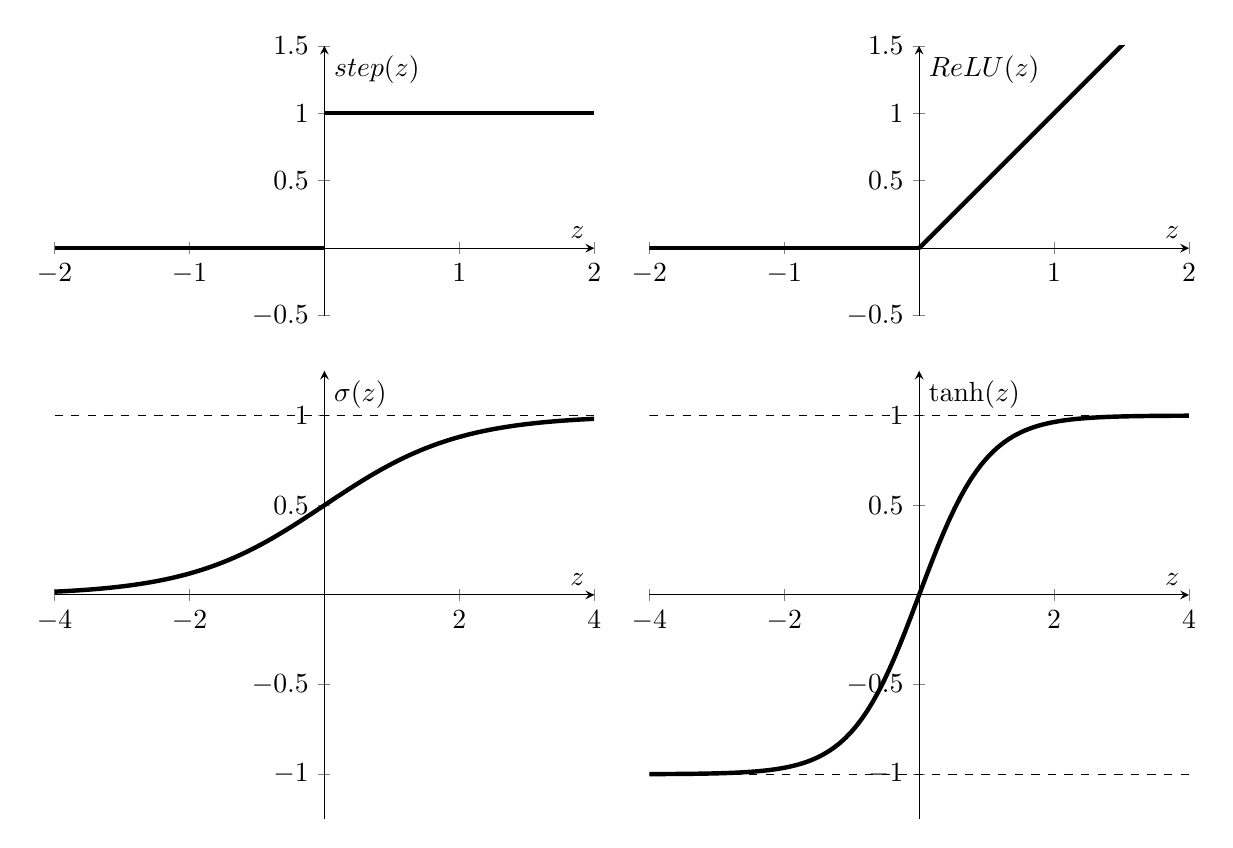
\begin{tikzpicture}%[scale=.9]
      \begin{axis}[
          name=topleft,
          axis lines=middle, axis equal image,
          xmin=-2, xmax=2,
          ymin=-.5, ymax=1.5,
          xlabel={$z$}, ylabel={$\text{step}(z)$},
        ]
        \addplot [domain=-2:0, samples=2, ultra thick] {0};
        \addplot [domain=0:2, samples=2, ultra thick] {1};
      \end{axis}

      \begin{axis}[
          name=topright,
          axis lines=middle, axis equal image,
          xmin=-2, xmax=2,
          ymin=-.5, ymax=1.5,
          xlabel={$z$}, ylabel={$\text{ReLU}(z)$},
          at = (topleft.east), anchor=west, xshift=.7cm
        ]
        \addplot [domain=-2:0, samples=2, ultra thick] {0};
        \addplot [domain=0:2, samples=2, ultra thick] {x};
      \end{axis}

      \begin{axis}[
          name=bottomleft,
          axis lines=middle, %axis equal image,
          xmin=-4, xmax=4,
          ymin=-1.25, ymax=1.25,
          xlabel={$z$}, ylabel={$\sigma(z)$},
          at = (topleft.south), anchor=north, yshift=-.7cm
        ]
        \addplot [domain=-4:4, samples=100, ultra thick] {1/(1+exp(-x))};
        \addplot [domain=-4:4, samples=2, dashed] {1};
        \addplot [domain=-4:4, samples=2, dashed] {0};
      \end{axis}

      \begin{axis}[
          name=bottomright,
          axis lines=middle, %axis equal image,
          xmin=-4, xmax=4,
          ymin=-1.25, ymax=1.25,
          xlabel={$z$}, ylabel={$\tanh(z)$},
          at = (bottomleft.east), anchor=west, xshift=.7cm
        ]
        \addplot [domain=-4:4, samples=100, ultra thick]
        {(exp(x) - exp(-x))/(exp(x) + exp(-x))};
        \addplot [domain=-4:4, samples=2, dashed] {1};
        \addplot [domain=-4:4, samples=2, dashed] {-1};
      \end{axis}
    \end{tikzpicture}
  }%
\end{center}

The original idea for neural networks involved using the {\bf step}
function as an activation, but because the derivative of the
step function is zero everywhere except at the discontinuity
(and there it is undefined), gradient-descent methods won't be useful
in finding a good setting of the weights, and so we won't
consider them further.  They have been replaced, in a sense, by the
sigmoid, ReLU, and tanh activation functions.
\question{
  Consider sigmoid, ReLU, and tanh activations.  Which one is most like
  a step function?  Is there an additional parameter you could add to a
  sigmoid that would make it be more like a step function?
}
\question{
  What is the derivative of the ReLU function?  Are there some values of
  the input for which the derivative vanishes?
}

ReLUs are especially common in internal (``hidden'') layers, 
sigmoid activations are common for the output for binary
classification, and softmax activations are common for the output for multi-class classification
(see Section~\ref{logistic} for an explanation).

\section{Loss functions and activation functions}\index{neural network!loss and activation function choices}
Different loss functions make different assumptions about the range of
values they will get as input and, as we have seen, different
activation functions will produce output values in different ranges.
When you are designing a neural network, it's important to make these
things fit together well.  In particular, we will think about matching
loss functions with the activation function in the last layer, $f^L$.
Here is a table of loss functions and activations that make sense for them:
\begin{center}
  \begin{tabular}{c c l}
    Loss       & $f^L$   & task                       \\
    \hline
    squared    & linear  & regression                 \\
    %  hinge & linear \\
    {\sc nll}  & sigmoid & binary classification             \\
    {\sc nllm} & softmax & multi-class classification
  \end{tabular}
\end{center}
We explored squared loss in Chapter~\ref{chap-regression} and ({\sc nll} and {\sc nllm}) in
Chapter~\ref{chap-classification}.

% \subsection{Two-class classification and log likelihood}
% For classification, the natural loss function is 0-1 loss, but we have
% already discussed the fact that it's very inconvenient for
% gradient-based learning because its derivative is discontinuous.

% It is nice
% and smooth, and extends nicely to multiple classes as we will see below.

% {\em Hinge loss} gives us another way, for binary classification
% problems, to make a smoother objective, penalizing the {\em margin}s
% of the labeled points relative to the separator.  The hinge loss is
% defined to be
% \[\mathcal{L}_h(\text{guess},\text{actual}) = \max(1 - \text{guess} \cdot
%   \text{actual}, 0)\;\;,\]
% when $\text{actual} \in \{+1, -1\}$.  It has the property that, if the
% sign of $\text{guess}$ is the same as the sign of $\text{actual}$ and the
% magnitude of $\text{guess}$ is greater than $1$, then the loss is 0.

% It is trying to enforce not only that the guess have the correct sign,
% but also that it should be some distance away from the separator.
% Using hinge loss, together with a squared-norm regularizer, actually
% forces the learning process to try to find a separator that has the
% maximum {\em margin} relative to the data set.  This optimization
% set-up is called a {\em support vector machine}, and was popular
% before the renaissance of neural networks and gradient descent,
% because it has a quadratic form that makes it particularly easy to
% optimize.



% Let's assume that the activation function on the output layer is a
% sigmoid and that there is a single unit in the output layer, so the
% output of the whole neural network is a scalar, $a^L$.  Because $f^L$
% is a sigmoid, we know $a^L \in [0, 1]$, and we can interpret it as the
% probability that  the input $x$ is a positive example.  Let  us
% further assume that the labels in the training data are $y \in \{0,
% 1\}$, so they can also be interpreted  as probabilities.

% We might want to pick the parameters of our network to maximize the
% probability that the network assigns the correct labels  to all the
% points.  That would be
% \begin{equation*}
%  \prod_{i = 1}^n \begin{cases} \ex{a}{i} & \text{if $\ex{y}{i} =
%     1$}  \\ 1 - \ex{a}{i} & \text{otherwise}
% \end{cases}\;\;,
% \end{equation*}
% under the assumption that our predictions are independent.  This can
% be cleverly rewritten as
% \begin{equation*}
%  \prod_{i = 1}^n {\ex{a}{i}}^{\ex{y}{i}}(1 - \ex{a}{i})^{1 - \ex{y}{i}}\;\;.
% \end{equation*}
% \question{Be sure you can see why these two expressions are  the
%   same.}

% Now, because products are kind of hard to deal with, and because the
% log function is monotonic, the $W$ that maximizes the log of this
% quantity will be the same  as the $W$ that maximizes the original, so
% we can try to maximize
% \begin{equation*}
%  \sum_{i = 1}^n {\ex{y}{i}}\log {\ex{a}{i}} + (1 - \ex{y}{i})\log(1 -
%  \ex{a}{i})\;\;,
% \end{equation*}
% which we can write in terms of a loss function
% \begin{equation*}
%  \sum_{i = 1}^n \mathcal{L}_\text{nll}(\ex{a}{i}, \ex{y}{i})
% \end{equation*}
% where $\mathcal{L}_\text{nll}$ is the {\em negative log likelihood}
% loss function:
% \begin{equation*}
% \mathcal{L}_\text{nll}(\text{guess},\text{actual}) =
% -\left(\text{actual}\cdot \log (\text{guess}) + (1 - \text{actual})\cdot\log (1 -
%   \text{guess})\right) \;\;.
% \end{equation*}
% This loss function is also sometimes referred to as the {\em log loss}
% or {\em cross entropy}. \note{You can use any base for the logarithm
%   and it won't make any real difference.  If we ask you for numbers,
%   use log base $e$.}

% \subsection{Multi-class classification and log likelihood}
% We can extend the idea of NLL directly to multi-class classification with
% $K$ classes, where the training label is represented with the one-hot
% vector
% $y=\begin{bmatrix} y_1,  \ldots, y_K \end{bmatrix}^T$, where $y_k=1$
% if the example is of class $k$. Assume that our network uses {\em
%   softmax} as the activation function in the last layer, so that the
% output is
% $a=\begin{bmatrix} a_1, \ldots, a_K
% \end{bmatrix}^T$, which represents a probability distribution over
% the $K$ possible classes. Then, the probability that our network
% predicts the correct class for this example is
% $\prod_{k=1}^K a_k^{y_k}$ and the log of the probability that it is
% correct is $\sum_{k=1}^K y_k \log a_k$, so
% \[
% \mathcal{L}_\text{nllm}(\text{guess},\text{actual}) =
% - \sum_{k=1}^K \text{actual}_k \cdot \log(\text{guess}_k) \;\;.
% \]
% We'll call this {\sc nllm} for {\em negative log likelihood
%   multiclass.}
% \question{Show that $L_\text{nllm}$ for  $K = 2$ is the same as
%   $L_\text{nll}$. }

%%%%%%%%%%%%%%%%%%%%%%%%%%%%%%%%%%%%%%%%

\section{Error back-propagation}
We will train neural networks using gradient descent methods.\index{gradient descent!applied to neural network training}  It's
possible to use {\em batch} gradient descent, in which we sum up the
gradient over all the points (as in Section~\ref{sec-gd} of
chapter~\ref{chap-gradient}) or
stochastic gradient descent ({\sc sgd}), in which we take a small step with
respect to the gradient considering a single point at a time (as in
Section~\ref{sec-sgd} of Chapter~\ref{chap-gradient}).

Our notation is going to get pretty hairy pretty quickly.  To keep it
as simple as we can, we'll focus on computing the contribution of one
data point $\ex{x}{i}$ to the gradient of the loss with respect to the
weights, for {\sc sgd}; you can simply sum up these gradients over all
the data points if you wish to do batch descent.

So, to do {\sc sgd} for a training example $(x, y)$, we need to
compute $\nabla_W \mathcal{L}(\text{NN}(x;W),y)$,
where $W$ represents all weights $W^l, W_0^l$ in all the layers $l =
  (1, \ldots, L)$. This seems terrifying,
but is actually quite easy to do using the chain rule.
\note{Remember the chain rule!  If $a = f(b)$ and $b = g(c)$, so that\\
  $a = f(g(c))$, then \\$\frac{d a}{d c} = \frac{d a}{d b} \cdot \frac{d
    b}{d c} = f'(b) g'(c) = f'(g(c)) g'(c)$.}

Remember that we are always computing the gradient of the loss
function {\em with respect to the weights} for a particular value of
$(x,  y)$.  That tells us how much we want to change the weights, in
order to reduce the loss incurred on this particular training example.

\subsection{First, suppose everything is one-dimensional}

To get some intuition for how these derivations work, we'll first suppose everything in our neural network is one-dimensional.
In particular, we'll assume there are $m^l = 1$ inputs and $n^l = 1$ outputs at every layer. So layer $l$ looks like:
\[
  a^l = f^l(z^l), \quad z^l = w^l a^{l-1} + w^l_0.
\]
In the equation above, we're using the lowercase letters $a^l, z^l, w^l, a^{l-1}, w^l_0$ to emphasize that all of these quantities are scalars just for the moment. We'll look at the more general matrix case below.

To use {\sc sgd}, then, we want \note{Check your understanding: why do we need exactly these quantities for SGD?} to compute $\partial \mathcal{L}(\text{NN}(x;W),y) / \partial w^l$ and $\partial \mathcal{L}(\text{NN}(x;W),y) / \partial w_0^l$ for each layer $l$ and each data point $(x,y)$. Below we'll write ``loss'' as an abbreviation for $\mathcal{L}(\text{NN}(x;W),y)$. Then our first quantity of interest is $\partial \text{loss} / \partial w^l$. The chain rule gives us the following.
First, let's look at the case $l=L$:
\begin{eqnarray*}
  \frac{ \partial \text{loss} }{ \partial w^L }
  &=& \frac{ \partial \text{loss} }{ \partial a^L }
  \cdot \frac{ \partial a^L }{ \partial z^L }
  \cdot \frac{ \partial z^L }{ \partial w^L } \\
  &=& \frac{ \partial \text{loss} }{ \partial a^L } \cdot (f^L)'(z^L) \cdot a^{L-1}.
\end{eqnarray*}
Now we can look at the case of general $l$:
\begin{eqnarray*}
  \frac{ \partial \text{loss} }{ \partial w^l }
  &=& \frac{ \partial \text{loss} }{ \partial a^L }
  \cdot \frac{ \partial a^L }{ \partial z^L }
  \cdot \frac{ \partial z^L }{ \partial a^{L-1} }
  \cdot \frac{ \partial a^{L-1} }{ \partial z^{L-1} }
  \cdots
  %\frac{ \partial a^{l+1} }{ \partial z^{l+1} }
  \frac{ \partial z^{l+1} }{ \partial a^{l} }
  \cdot \frac{ \partial a^{l} }{ \partial z^l }
  \cdot \frac{ \partial z^l }{ \partial w^l } \\
  &=& \frac{ \partial \text{loss} }{ \partial a^L } \cdot (f^L)'(z^L) \cdot w^L
  \cdot (f^{L-1})'(z^{L-1})
  \cdots
  %\cdot (f^{l+1})'(z^{l+1})
  \cdot w^{l+1}
  \cdot (f^{l})'(z^{l})
  \cdot a^{l-1} \\
  &=& \frac{ \partial \text{loss} }{ \partial z^l } \cdot a^{l-1}.
\end{eqnarray*}

Note that every multiplication above is scalar multiplication because every term in every product above is a scalar. And though we solved for all the other terms in the product, we haven't solved for $\partial \text{loss} / \partial a^L$ because the derivative will depend on which loss function you choose. Once you choose a loss function though, you should be able to compute this derivative.

\question{Suppose you choose squared loss. What is $\partial \text{loss} / \partial a^L$?}

\question{Check the derivations above yourself. You should use the chain rule and also solve for the individual derivatives that arise in the chain rule.}

\question{Check that the the final layer ($l=L$) case is a special case of the general layer $l$ case above.}

\question{Derive $\partial \mathcal{L}(\text{NN}(x;W),y) / \partial w_0^l$ for yourself, for both the final layer ($l=L$) and general $l$.}

\question{Does the $L=1$ case remind you of anything from earlier in this course?}

\question{Write out the full SGD algorithm for this neural network.}

It's pretty typical to run the chain rule from left to right like we did above. But, for where we're going next, it will be useful to notice that it's completely equivalent to write it in the other direction. So we can rewrite our result from above as follows:
\begin{eqnarray}
  \label{eq:gradloss_oned}
  \frac{ \partial \text{loss} }{ \partial w^l }
  &=& a^{l-1} \cdot \frac{ \partial \text{loss} }{ \partial z^l } \\
  \label{eq:gradz_intermediate_oned}
  \frac{ \partial \text{loss} }{ \partial z^l }
  &=& \frac{ \partial a^{l} }{ \partial z^l }
  \cdot \frac{ \partial z^{l+1} }{ \partial a^{l} }
  \cdots
  \frac{ \partial a^{L-1} }{ \partial z^{L-1} }
  \cdot \frac{ \partial z^L }{ \partial a^{L-1} }
  \cdot \frac{ \partial a^L }{ \partial z^L }
  \cdot \frac{ \partial \text{loss} }{ \partial a^L } \\
  \label{eq:gradz_oned}
  &=& \frac{ \partial a^{l} }{ \partial z^l } \cdot w^{l+1}
  \cdots
  \frac{ \partial a^{L-1} }{ \partial z^{L-1} } \cdot w^L \cdot \frac{ \partial a^L }{ \partial z^L }
  \cdot \frac{ \partial \text{loss} }{ \partial a^L }.
\end{eqnarray}


\subsection{The general case}

Next we're going to do everything that we did above, but this time we'll allow any number of inputs $m^l$ and outputs $n^l$ at every layer. First, we'll tell you the results that correspond to our derivations above. Then we'll talk about why they make sense. And finally we'll derive them carefully.

OK, let's start with the results! Again, below we'll be using ``loss'' as an abbreviation for $\mathcal{L}(\text{NN}(x;W),y)$. Then,
\begin{eqnarray}
  \label{eq:gradloss}
  \underbrace{\frac{\partial \text{loss}}{\partial W^l}}_{m^l \times n^l}
  &=&
  \underbrace{A^{l-1}}_{m^l \times 1} \;
  \underbrace{\left(\frac{\partial \text{loss}}{\partial
      Z^l}\right)^T}_{1 \times n^l} \\
  %
  \label{eq:gradz_intermediate}
  \frac{\partial \text{loss}}{\partial Z^l}
  &=& \frac{\partial A^l}{\partial Z^l}
  %%\cdot \frac{\partial Z^l}{ \partial A^{l+1}}
  \cdot \frac{\partial Z^{l+1}}{ \partial A^l}
  %\cdot \frac{\partial A^{l+1}}{\partial Z^{l+1}}
  \cdots
  %\cdot \frac{\partial Z^{L-1}}{\partial A^{L-2}}
  \cdot \frac{\partial A^{L-1}}{\partial Z^{L-1}}
  \cdot \frac{\partial Z^{L}}{\partial A^{L-1}}
  \cdot \frac{\partial A^{L}}{\partial Z^{L}}
  \cdot \frac{\partial \text{loss}}{\partial A^L}
  \\
  \label{eq:gradz}
  &=& \frac{\partial A^l}{\partial Z^l}
  \cdot W^{l+1}
  % \cdot W^l
  %\cdot \frac{\partial A^{l+1}}{\partial Z^{l+1}}
  \cdots
  %W^{L-1}
  \cdot \frac{\partial A^{L-1}}{\partial Z^{L-1}}
  \cdot W^{L}
  \cdot \frac{\partial A^{L}}{\partial Z^{L}}
  \cdot \frac{\partial \text{loss}}{\partial A^L} \; .
\end{eqnarray}

First, compare each equation to its one-dimensional counterpart, and make sure you see the similarities.
That is, compare the general weight derivatives in Eq.~\ref{eq:gradloss} to the one-dimensional case in Eq.~\ref{eq:gradloss_oned}. Compare the intermediate derivative of loss with respect to the pre-activations $Z^l$ in Eq.~\ref{eq:gradz_intermediate} to the one-dimensional case in Eq.~\ref{eq:gradz_intermediate_oned}. And finally compare the version where we've substituted in some of the derivatives in Eq.~\ref{eq:gradz} to Eq.~\ref{eq:gradz_oned}. Hopefully you see how the forms are very analogous. But in the matrix case, we now have to be careful about the matrix dimensions. We'll check these matrix dimensions below.

Let's start by talking through each of the terms in the matrix version of these equations. Recall that loss is a scalar, and $W^l$ is a matrix of size $m^l \times n^l$. You can read about the conventions in the course for derivatives starting in this chapter in Appendix~\ref{app:matrix_deriv}. By these conventions (not the only possible conventions!), we have that $\partial \text{loss} / \partial W^l$ will be a matrix of size $m^l \times n^l$ whose $(i,j)$ entry is the scalar $\partial \text{loss} / \partial W^l_{i,j}$. In some sense, we're just doing a bunch of traditional scalar derivatives, and the matrix notation lets us write them all simultaneously and succinctly. In particular, for SGD, we need to find the derivative of the loss with respect to every scalar component of the weights because these are our model's parameters and therefore are the things we want to update in SGD.

The next quantity we see in Eq.~\ref{eq:gradloss} is $A^{l-1}$, which we recall has size $m^l \times 1$ (or equivalently $n^{l-1} \times 1$ since it represents the outputs of the $l-1$ layer). Finally, we see $\partial \text{loss} / \partial Z^l$. Again, loss is a scalar, and $Z^l$ is a $n^l \times 1$ vector. So by the conventions in Appendix~\ref{app:matrix_deriv}, we have that $\partial \text{loss} / \partial Z^l$ has size $n^l \times 1$. The transpose then has size $1 \times n^l$. Now you should be able to check that the dimensions all make sense in Eq.~\ref{eq:gradloss}; in particular, you can check that inner dimensions agree in the matrix multiplication and that, after the multiplication, we should be left with something that has the dimensions on the lefthand side.

Now let's look at Eq.~\ref{eq:gradz}. We're computing $\partial \text{loss} / \partial Z^l$ so that we can use it in Eq.~\ref{eq:gradloss}. The weights are familiar. The one part that remains is terms of the form $\partial A^l / \partial Z^l$. Checking out Appendix~\ref{app:matrix_deriv}, we see that this term should be a matrix of size $n^l \times n^l$ since $A^l$ and $Z^l$ both have size $n^l \times 1$. The $(i,j)$ entry of this matrix is $\partial A^l_j / \partial Z^l_i$. This scalar derivative is something that you can compute when you know your activation function. If you're not using a softmax activation function, $A^l_j$ typically is a function only of $Z^l_j$, which means that $\partial A^l_j / \partial Z^l_i$ should equal 0 whenever $i \ne j$, and that $\partial A^l_j / \partial Z^l_j = (f^l)'(Z^l_j)$.

\question{Compute the dimensions of every term in Eqs.~\ref{eq:gradz_intermediate} and \ref{eq:gradz} using Appendix~\ref{app:matrix_deriv}. After you've done that, check that all the matrix multiplications work; that is, check that the inner dimensions agree and that the lefthand side and righthand side of these equations have the same dimensions.}

\question{If I use the identity activation function, what is $\partial A^l_j / \partial Z^l_j$ for any $j$? What is the full matrix $\partial A^l / \partial Z^l$?}

\subsection{Derivations for the general case}

You can use everything above without deriving it yourself. But if you want to find the gradients of loss with respect to $W^l_0$ (which we need for SGD!), then you'll want to know how to actually do these derivations. So next we'll work out the derivations.

The key trick is to just break every equation down into its scalar meaning. For instance, the $(i,j)$ element of $\partial \text{loss} / \partial W^l$ is $\partial \text{loss} / \partial W^l_{i,j}$. If you think about it for a moment (and it might help to go back to the one-dimensional case), the loss is a function of the elements of $Z^l$, and the elements of $Z^l$ are a function of the $W^l_{i,j}$. There are $n^l$ elements of $Z^l$, so we can use the chain rule to write
\begin{equation}
  \label{eq:partial_loss_partial_W_intermediate}
  \frac{ \partial \text{loss} }{ \partial W^l_{i,j} }
  = \sum_{k=1}^{n^l} \frac{ \partial \text{loss} }{ \partial Z^l_k } \frac{ \partial Z^l_k }{ \partial W^l_{i,j} }.
\end{equation}
To figure this out, let's remember that $Z^l = (W^l)^\top A^{l-1} + W_0^l$. We can write one element of the $Z^l$ vector, then, as $Z^l_{b} = \sum_{a=1}^{m^l} W_{a,b}^{l} A_a^{l-1} + (W_0^l)_b$. It follows that $\partial Z^l_k / \partial W^l_{i,j}$ will be zero except when $k=j$ (check you agree!). So we can rewrite Eq.~\ref{eq:partial_loss_partial_W_intermediate} as
\begin{equation}
  \label{eq:partial_loss_partial_W_entries}
  \frac{ \partial \text{loss} }{ \partial W^l_{i,j} }
  = \frac{ \partial \text{loss} }{ \partial Z^l_j } \frac{ \partial Z^l_j }{ \partial W^l_{i,j} }
  = \frac{ \partial \text{loss} }{ \partial Z^l_j } A_i^{l-1}.
\end{equation}
Finally, then, we match entries of the matrices on both sides of the equation above to recover Eq.~\ref{eq:gradloss}.

\question{Check that Eq.~\ref{eq:partial_loss_partial_W_entries} and Eq.~\ref{eq:gradloss} say the same thing.}

\question{Convince yourself that $\partial Z^{l} / \partial A^{l-1} = W^l$ by comparing the entries of the matrices on both sides on the equality sign.}

\question{Convince yourself that Eq.~\ref{eq:gradz_intermediate} is true.}

\question{Apply the same reasoning to find the gradients of
  $\text{loss}$ with respect to $W_0^l$.}

\subsection{Reflecting on backpropagation}

This general process of computing the gradients of the loss with respect to the weights
is called {\em error back-propagation}.\index{error back-propagation}
\note{We could call this
  ``blame propagation''.  Think of $\text{loss}$ as how mad we
  are about the prediction just made.  Then $\partial
    \text{loss}/ \partial A^L$ is how much we blame $A^L$ for the loss.
  The last module has to take in $\partial \text{loss}/ \partial A^L$
  and compute $\partial \text{loss}/ \partial Z^L$, which is how much
  we blame $Z^L$ for the loss.  The next module (working backwards)
  takes in $\partial \text{loss}/ \partial Z^L$ and computes $\partial
    \text{loss}/ \partial A^{L-1}$.  So every module is accepting its
  blame for the loss, computing how much of it to allocate to each of
  its inputs, and passing the blame back to them.}
The idea
is that we first do a {\em forward pass} to compute all the $a$ and
$z$ values at all the layers, and finally the actual loss.  Then, we can work backward and compute the gradient of the
loss with respect to the weights in each layer, starting at layer $L$
and going back to layer 1.

\begin{center}
  \begin{tikzpicture}[scale=.98]
    \coordinate (x) at (0,0);
    \node[inner sep=0em] (w1) at (1.7,0)
    {\begin{tabular}{c} $W^1$ \\ $W^1_0$\end{tabular}};
    \node[inner sep=1em] (f1) at ($2*(w1)$) {$f^1$};
    \node[inner sep=0em] (w2) at ($3*(w1)$)
    {\begin{tabular}{c} $W^2$ \\ $W^2_0$\end{tabular}};
    \node[inner sep=1em] (f2) at ($4*(w1)$) {$f^2$};
    \node (dots) at ($5*(w1)$) {$\cdots$};
    \node[inner sep=0em] (wL) at ($6*(w1)$)
    {\begin{tabular}{c} $W^L$ \\ $W^L_0$\end{tabular}};
    \node[inner sep=1em] (fL) at ($7*(w1)$) {$f^L$};
    \node (loss) at ($8*(w1)$) {Loss};
    \coordinate (y) at ($8*(w1) + (0,1.5)$);

    \draw[->] (x) -- node[above] {$X = A^0$} (w1);
    \draw[->] (w1) -- node[above] {$Z^1$} (f1);
    \draw[->] (f1) -- node[above] {$A^1$} (w2);
    \draw[->] (w2) -- node[above] {$Z^2$} (f2);
    \draw[->] (f2) -- node[above] {$A^2$} (dots);
    \draw[->] (dots) -- node[above] {$A^{L-1}$} (wL);
    \draw[->] (wL) -- node[above] {$Z^L$} (fL);
    \draw[->] (fL) -- node[above] {$A^L$} (loss);
    \draw[->] (y) -- node[right] {$y$} ($(loss)+(0,.65)$);

    %\draw[->,yshift=0.5cm] (loss.west) to [out=150,in=30] (fL.east);
    \foreach \s/\e/\t in {loss/fL/A^L,
    fL/wL/Z^L,
    wL/dots/A^{L-1},
    dots/f2/A^2,
    f2/w2/Z^2,
    w2/f1/A^1,
    f1/w1/Z^1}{
    \path[->] ($(\s.west) - (0,.5)$) edge[out=210,in=-30] node[below]
      {$\frac{\partial \text{loss}}{\partial \t}$}
    ($(\e.east) - (0,.5)$);
    }
    \foreach \point in {w1, f1, w2, f2, wL, fL}{
        \draw ($(\point) + (-.3,-.5)$) rectangle ($(\point) + (.3,.5)$);
      }
    \draw ($(loss) + (-.4,-.5)$) rectangle ($(loss) + (.4,.5)$);
  \end{tikzpicture}
\end{center}

If we view our neural network as a sequential composition of modules
(in our work so far, it has been an alternation between a linear
transformation with a weight matrix, and a component-wise application
of a non-linear activation function), then we can define a simple API
for a module that will let us compute the forward and backward passes,
as well as do the necessary weight updates for gradient descent.  Each
module has to provide the following ``methods.''  We are already using
letters $a, x, y, z$ with particular meanings, so here we will use $u$
as the vector input to the module and $v$ as the vector output:
\begin{itemize}
  \item forward: $u \rightarrow v$
  \item backward: $u, v, \partial L /
          \partial v \rightarrow \partial L / \partial u$
  \item weight grad: $u, \partial L / \partial v \rightarrow \partial L
          / \partial W$  only needed for modules that have weights $W$
\end{itemize}
In homework we will ask you to implement these modules for neural
network components, and then use them to construct a network and train
it as described in the next section.

% \begin{examplebox}
% What are some conventions for derivatives of matrices and vectors?  It
% will always work to explicitly write all indices and treat everything
% as scalars, but we introduce here some shortcuts that are often faster
% to use and helpful for understanding:
% \begin{itemize}

% \item For $v$ of size $1\times 1$ and $u$ of size $1\times 1$,
%   $\partial v/\partial u$ is the (scalar) partial derivative of $v$
%   w.r.t. $u$.  Example: $\underbrace{\partial L}_{1\times
%     1}/\underbrace{\partial W}_{1\times 1}$ is $1\times 1$

% \item For $v$ of size $1\times 1$ and $u$ of size $b\times 1$,
%   $\partial v/\partial u$ is a vector of size $b\times 1$ with the $j^{\rm th}$ entry $\partial v/\partial u_j$.
%   Example: $\underbrace{\partial L}_{1\times 1}/\underbrace{\partial W_0}_{n\times 1}$ is $n\times 1$

% \item For $v$ of size $c\times 1$ and $u$ of size $b\times 1$,
%   $\partial v/\partial u$ is a vector of size $b\times c$ with the $(j, k)$ entry $\partial v_k/\partial u_j$.
%   Example: $\underbrace{\partial A}_{n\times 1}/\underbrace{\partial Z}_{n\times 1}$ is $n\times n$

% \item For $v$ of size $1\times 1$ and $u$ of size $b\times c$,
%   $\partial v/\partial u$ is a vector of size $b\times c$ with the $(j, k)$ entry $\partial v/\partial u_{j,k}$.
%   Example: $\underbrace{\partial L}_{1\times 1}/\underbrace{\partial W}_{m\times n}$ is $m\times n$

% \end{itemize}
% \end{examplebox}



%\chapter{Making NN's Work}
\section{Training}
Here we go!  Here's how to do stochastic gradient descent training on
a feed-forward neural network.\index{neural network!training}   After this pseudo-code, we motivate
the choice of initialization in lines 2 and 3.  The actual
computation of the gradient values (e.g., $\partial\text{loss}/
  \partial A^L$) is not directly defined in this code, because we want
to make the structure of the computation clear.
\question{What is $\partial Z^l / \partial W^l$? }
\question{Which terms in the code below depend on $f^L$?}

\begin{codebox}
  \Procname{$\proc{SGD-Neural-Net}(\dataTrain, T, L, (m^1, \ldots,
    m^L), (f^1, \ldots, f^L), \text{Loss})$}
    \li     \For $l \gets 1$ \To $L$
    \Do
    \li        $W_{ij}^l \sim \text{Gaussian}(0, 1/m^l)$
    \li        $W_{0j}^l \sim \text{Gaussian}(0, 1)$
    \End
    \li \For $t \gets 1$ \To $T$
    \li   \Do
  $i \gets \text{random sample from } \{1,\ldots,n\}$
    \li     $A^0 \gets \ex{x}{i}$
    \li     \Comment forward pass to compute the output $A^L$
    \li     \For $l \gets 1$ \To $L$
    \li       \Do
  $Z^l \gets W^{l^T}A^{l-1} + W_0^l$
    \li         $A^l \gets f^l(Z^l)$
    \End
    \li     $\text{loss} \gets \text{Loss}(A^L, \ex{y}{i})$
    \li     \For $l \gets L$ \To 1:
    \Do
    \li       \Comment error back-propagation
    \li       $\partial \text{loss}/\partial A^l \gets$ 	%
    %            m x 1
    {\bf if} $l < L$
    {\bf then}
    % dims:          n x 1                    *    m x n
  $\partial Z^{l+1}/\partial A^l \cdot \partial \text{loss}/\partial Z^{l+1} $
    % dims:  m x n                   *     n x 1
    {\bf else}
  $ \partial \text{loss}/\partial A^L$
    \li       $\partial \text{loss}/\partial Z^l \gets \partial
  A^l/\partial Z^l  \cdot \partial
  \text{loss}/\partial A^l$
    \li       \Comment compute gradient with respect to weights
    \li       $\partial \text{loss}/\partial W^l  \gets        A^{l-1}      \cdot    \left( \partial \text{loss}/\partial Z^l  \right)^T $
    %                           m x n              =            m x 1          *        1 x n
    \li       $\partial \text{loss}/\partial W_0^l \gets       \partial \text{loss}/\partial Z^l $
    %                           1 x n              =                  1 x n
    \li       \Comment stochastic gradient descent update
    \li       $W^l = W^l - \eta(t)\cdot \partial \text{loss}/\partial W^l$
    \li       $W^l_0 = W_0^l - \eta(t)\cdot \partial \text{loss}/\partial W_0^l$
  \End
\end{codebox}

Initializing $W$ is important;\index{neural network!initialization of weights}  if you do it badly there is a good
chance the neural network training won't work well.  First, it is
important to initialize the weights to random values.  We want
different parts of the network to tend to ``address'' different
aspects of the problem; if they all start at the same weights, the
symmetry will often keep the values from moving in useful directions.
Second, many of our activation functions have (near) zero slope when
the pre-activation $z$ values have large magnitude, so we generally
want to keep the initial weights small so we will be in a situation
where the gradients are non-zero, so that gradient descent will have
some useful signal about which way to go.

One good general-purpose strategy is to choose each weight at random
from a Gaussian (normal) distribution with mean 0 and standard
deviation $(1/m)$ where $m$ is the number of inputs to the unit.
\question{If the input $x$ to this unit is a vector of 1's, what would
  the expected pre-activation $z$ value be with these initial
  weights?}  We write this choice (where $\sim$ means ``is drawn
randomly from the distribution'') as $W^l_{ij} \sim \text{Gaussian}\left(0,
  \frac{1}{m^l}\right).$ It will often turn out (especially for fancier activations and loss
functions) that computing
$\frac{\partial \text{loss}}{\partial Z^L}$ is easier than computing
$\frac{\partial \text{loss}}{\partial A^L}$ and $\frac{\partial A^L}{\partial Z^L}.$ So, we may instead ask for an implementation of a loss function to provide a backward method that computes $\partial \text{loss}/\partial Z^L$ directly.


\section{Optimizing neural network parameters}
\label{sec-make_nn_work}

Because neural networks are just parametric functions, we can optimize
loss with respect to the parameters using standard gradient-descent
software, but we can take advantage of the structure of the loss
function and the hypothesis class to improve optimization.  As we have
seen, the modular function-composition structure of a neural network
hypothesis makes it easy to organize the computation of the gradient.
As we have also seen earlier, the structure of the loss function as a
sum over terms, one per training data point, allows us to consider
stochastic gradient methods.  In this section we'll consider some
alternative strategies for organizing training, and also for making it
easier to handle the step-size parameter.

\subsection{Batches}
Assume that we have an objective of the form
\[J(W) = \sum_{i = 1}^n \mathcal{L}(h(\ex{x}{i}; W),  \ex{y}{i})\;\;,\]
where $h$ is the function computed by a neural network, and $W$ stands
for all the weight matrices and vectors in the network.

Recall that, when we perform {\em batch} (or the vanilla) gradient descent, we use the update rule
\[W_t = W_{t-1} - \eta\nabla_W J(W_{t-1})\;\;,\]
which is equivalent to
\[W_t = W_{t-1} - \eta\sum_{i=1}^n \nabla_W \mathcal{L}(h(\ex{x}{i}; W_{t-1}),
  \ex{y}{i})\;\;.\]
So, we sum up the gradient of loss at each training point,  with
respect to $W$, and then take a step in the negative direction of
the gradient.

In {\em stochastic} gradient descent, we repeatedly pick a point
$(\ex{x}{i}, \ex{y}{i})$ at random from the data set, and execute a
weight update on that point alone:
\[W_t = W_{t-1} - \eta \nabla_W \mathcal{L}(h(\ex{x}{i}; W_{t-1}),
  \ex{y}{i})\;\;.\]
As long as we pick points uniformly at random from the data set, and
decrease $\eta$ at an appropriate rate, we are guaranteed, with high
probability, to converge to at least a local optimum.

These two methods have offsetting virtues.  The batch method takes
steps in the exact gradient direction but requires a lot of
computation before even a single step can be taken, especially if the
data set is large.  The stochastic method begins moving right away,
and can sometimes make very good progress before looking at even a
substantial fraction of the whole data set, but if there is a lot of
variability in the data, it might require a very small $\eta$ to
effectively average over the individual steps moving in ``competing''
directions.

An effective strategy is to ``average'' between batch and stochastic
gradient descent by using {\em mini-batches}.  For a mini-batch of
size $K$, we select $K$ distinct data points uniformly at random from the data
set and do the update based just on their contributions to the gradient
\[W_t = W_{t-1} - \eta\sum_{i=1}^K \nabla_W \mathcal{L}(h(\ex{x}{i}; W_{t-1}),
  \ex{y}{i})\;\;.\]
Most neural network software packages are set up to do mini-batches.
\question{For what value of $K$ is mini-batch gradient descent
  equivalent to stochastic gradient descent?  To batch gradient
  descent?}

Picking $K$ unique data points at random from a large data-set is
potentially computationally difficult.  An alternative strategy, if
you have an efficient procedure for randomly shuffling the data set
(or randomly shuffling a list of indices into the data set) is to
operate in a loop, roughly as follows:

\begin{codebox}
  \Procname{$\proc{Mini-Batch-SGD}$(NN, data, K)}
  \li     $n = $ length(data)
  \li     \While not done:
  \Do
  \li        $\proc{Random-Shuffle}$(data)
  \li        \For $i \gets 1$ \To $\lceil n/K \rceil$
  \Do
  \li           $\proc{Batch-Gradient-Update}$(NN, data$[(i - 1)K:iK]$)
  \End
  \End
\end{codebox}
See note on the ceiling\footnote{
  In line 4 of the algorithm above, $\lceil \cdot \rceil$ is known
  as the \emph{ceiling} function; it returns the smallest
  integer greater than or equal to its input. E.g., $\lceil 2.5 \rceil = 3$ and $\lceil 3 \rceil = 3$.}
function, for the case when $n/K$ is not an integer.

\subsection{Adaptive step-size}
Picking a value for $\eta$ is difficult and time-consuming.\index{adaptive step size}  If it's
too small, then convergence is slow and if it's too large, then we
risk divergence or slow convergence due to oscillation.  This problem
is even more pronounced in stochastic or mini-batch mode, because we
know we need to decrease the step size for the formal guarantees to
hold.

It's also true that, within a single neural network, we may well want
to have different step sizes.  As our networks become {\em deep} (with
increasing numbers of layers) we can find that magnitude of the
gradient of the loss with respect the weights in the last layer,
$\partial \text{loss} / \partial W_L$, may be substantially
different from the gradient of the loss with respect to the weights in
the first layer $\partial \text{loss} / \partial W_1$.  If you look
carefully at Eq.~\ref{eq:gradz}, you can see that the output
gradient is multiplied by all the weight matrices of the network and
is ``fed back'' through all the derivatives of all the activation
functions.  This can lead to a problem of {\em exploding}  or {\em
    vanishing} gradients\index{exploding (or vanishing) gradients}, in which the back-propagated gradient is much
too big or small to be used in an update rule with the same step size.

So, we can consider having an independent step-size parameter {\em for each
    weight}, and updating it based on a local view of how the gradient
updates have been going.\note{This section is very strongly influenced
by Sebastian Ruder's excellent blog posts on the topic:
{\tt\scriptsize ruder.io/ optimizing-gradient-descent}}
Some common strategies for this include \emph{momentum} (``averaging'' recent gradient updates), \emph{Adadelta} (take larger steps in parts of the space where $J(W)$ is nearly flat), and \emph{Adam} (which combines these two previous ideas). Details of these approaches are described in Appendix~\ref{adaptive-step-size-appendix}. 


\section{Regularization}\index{neural network!regularization}
So far, we have only considered optimizing loss on the training data
as our objective for neural network training.   But, as we have
discussed before, there is a risk of overfitting if we do this.  The
pragmatic fact is that,  in current deep neural networks, which tend to be very
large and to be trained with a large amount of data,  overfitting is
not a huge problem.  This runs counter to our current theoretical
understanding and the study of this question is a hot area of
research.  Nonetheless, there are several strategies for regularizing
a neural network, and they can sometimes be important.

\subsection{Methods related to ridge regression}

One group of strategies can, interestingly, be shown to have similar
effects to each other: early stopping, weight decay, and adding noise
to the training data. \note{Result is due to Bishop, described in his
  textbook and here {\tt\scriptsize doi.org/10.1162/ neco.1995.7.1.108}.}

Early stopping is the easiest to implement and is in fairly common
use.  The idea is to train on your training set, but at every {\em
    epoch} (a pass through the whole training set, or possibly more
frequently), evaluate the loss of the current $W$ on a {\em validation
    set}.  It will generally be the case that the loss on the training
set goes down fairly consistently with each iteration, the loss on the
validation set will initially decrease, but then begin to increase
again.  Once you see that the validation loss is systematically
increasing, you can stop training and return the weights that had the
lowest validation error.

Another common strategy is to simply penalize the norm of all the
weights, as we did in ridge regression.  This  method is known as {\em
    weight decay}\index{neural network!weight decay}, because when we take the gradient of the objective
$$ J(W) = \sum_{i = 1}^{n}\mathcal{L}(\text{NN}(x^{(i)}), y^{(i)}; W)
  + \lambda\|W\|^2 $$
we end up  with an update of the form
\begin{align*}
  W_t & = W_{t-1} -
  \eta\left(\left(\nabla_{W}\mathcal{L}(\text{NN}(x^{(i)}),
  y^{(i)}; W_{t-1})\right) + 2\lambda W_{t-1}\right)                                      \\
      & = W_{t-1}(1 - 2\lambda\eta) - \eta\left(\nabla_{W}\mathcal{L}(\text{NN}(x^{(i)}),
    y^{(i)}; W_{t-1})\right) \;\;.
\end{align*}
This rule has the form of first ``decaying'' $W_{t-1}$ by a factor of
$(1 - 2 \lambda \eta)$ and then taking a gradient step.

Finally, the same effect can be achieved by perturbing the $\ex{x}{i}$
values of the training data by adding a small amount of zero-mean
normally distributed noise before each gradient computation.  It makes
intuitive sense that it would be more difficult for the network to
overfit to particular training data if they are changed slightly on
each training step.

\subsection{Dropout}
Dropout\index{neural network!dropout} is a regularization method that was designed to work with deep
neural networks.  The idea behind it is, rather than perturbing the
data every time we train, we'll perturb the network!  We'll do this by
randomly, on each training step, selecting a set of units in each
layer and prohibiting them from participating.   Thus, all of the
units will have to take a kind of  ``collective'' responsibility for
getting the answer right, and will not be able to rely on any small
subset of the weights to do all the necessary computation.  This tends
also to make the network more robust to data perturbations.

During the training phase, for each training example, for each unit,
randomly with probability $p$ temporarily set $a^{\ell}_j = 0$. There
will be no contribution to the output and no gradient update for the
associated unit.
\question{
  Be sure you understand why, when using {\sc sgd}, setting an
  activation value to 0 will cause that unit's weights not to be updated
  on that iteration.
}

When we are done training and want to use the network to make
predictions, we multiply all weights by $p$ to achieve the same average
activation levels.

Implementing dropout is easy!  In the forward pass during training, we let
$$ a^{\ell} = f(z^{\ell}) * d^{\ell} $$
where $*$ denotes component-wise product and $d^{\ell}$ is a vector of
$0$'s and $1$'s drawn randomly with probability $p$.
The backwards pass depends on $a^{\ell}$, so we do not need to make
any further changes to the algorithm.

It is common to set $p$ to $0.5$, but this is something one might
experiment with to get good results on your problem and data.

% Dropout is no longer in common use, but it is still interesting to
% think about.

\subsection{Batch normalization}

Another strategy that seems to help with regularization and robustness
in training is {\em batch normalization}.  \index{neural network!batch normalization}
\note{For more  details see {\tt\scriptsize arxiv.org/abs/1502.03167}.}
It was originally
developed to address a problem of {\em covariate shift}:  that is, if
you consider the second layer of a two-layer neural network, the
distribution of its input values is changing over time as the first
layer's  weights change.  Learning when the input distribution is
changing is extra difficult:  you have to change your weights to
improve your predictions, but also just to compensate for a change in
your inputs  (imagine, for instance, that the magnitude of the inputs
to your layer is increasing over time---then your weights will have to
decrease, just to keep your predictions the same).

So, when training with mini-batches, the idea is to {\em standardize}
the input values for each mini-batch, just in the way that we did it
in Section~\ref{realFeatures} of Chapter~\ref{chap-features}, subtracting off the mean
and dividing by the standard deviation of each input dimension.  This
means that the scale of the inputs to each layer remains the same, no
matter how the weights in previous layers change.  However, this
somewhat complicates matters, because the computation of the weight
updates will need to take into account that we are performing this
transformation.  In the modular view, batch normalization can be seen
as a module that is applied to $z^l$, interposed after the product
with $W^l$ and before input to $f^l$.\note{We follow here the
  suggestion from the original paper of applying batch normalization
  before the activation function.  Since then it has been shown that,
  in some cases, applying it after works a bit better. But there
  aren't any definite findings on which works better and when.}

Although batch-norm was originally justified based on the problem of
covariate shift, it's not clear that that is actually why it seems to
improve performance.
Batch normalization can also end up having a regularizing effect for similar
reasons that adding noise and dropout do:  each mini-batch of data
ends up being mildly perturbed, which prevents the network from
exploiting very particular values of the data points.
For those interested, the equations for batch normalization, including a derivation of the forward pass and backward pass, are described in Appendix~\ref{batch-norm-appendix}.


%%% Local Variables:
%%% mode: latex
%%% TeX-master: "top"
%%% End:


%%%%%%%%%%%%%%%%%%%%%%%%%%%%%%%%%%%%%%%%%%%%%%%%%%%%%%%%%%%%%%%%%%%%%%%%%%%%%

%%% Local Variables:
%%% mode: latex
%%% TeX-master: "top"
%%% End:
